% +------------------------------------------------------------------------+
% | Skin_surface_3/doc_tex/Skin_surface_3/MarchingTetrahedra3.tex
% +------------------------------------------------------------------------+
% | 2005 Nico Kruithof
% | Marching tetrahedral algorithm
% | 
\RCSdef{\skinSurfaceRev}{$Id$}
\RCSdefDate{\skinSurfaceDate}{$Date$}
% +------------------------------------------------------------------------+

\section{Marching tetrahedra}
The marching tetrahedra algorithm, introduced in
\cite{cgal:tpg-rmtiise-99}, is used in the construction of the coarse
mesh isotopic to skin surface. This algorithm is of general use and
therefore also documented.

The marching tetrahedra algorithm extracts a mesh from a
triangulation.  First, it labels each vertex of the triangulation
either as inside or as outside. The vertices of the mesh are
constructed as the intersection point of the surface and an edge with
different vertex-labels. The faces of the mesh are defined by the
tetrahedra of the triangulation. Based on the number of
triangulation-vertices inside the surface, we can distinguish five
cases, two of which are redundant if we allow the exchange of inside
and outside. In the case that all four labels are equal, the
tetrahedron does not contain a part of the surface. If three labels
are equal, the three vertices of the mesh form a triangle. If two
labels are equal, we construct two triangles. These three cases are
depicted in Figure~\ref{SkinSurface3-fig-marching}.

\begin{figure}
\begin{ccTexOnly}
\begin{center}
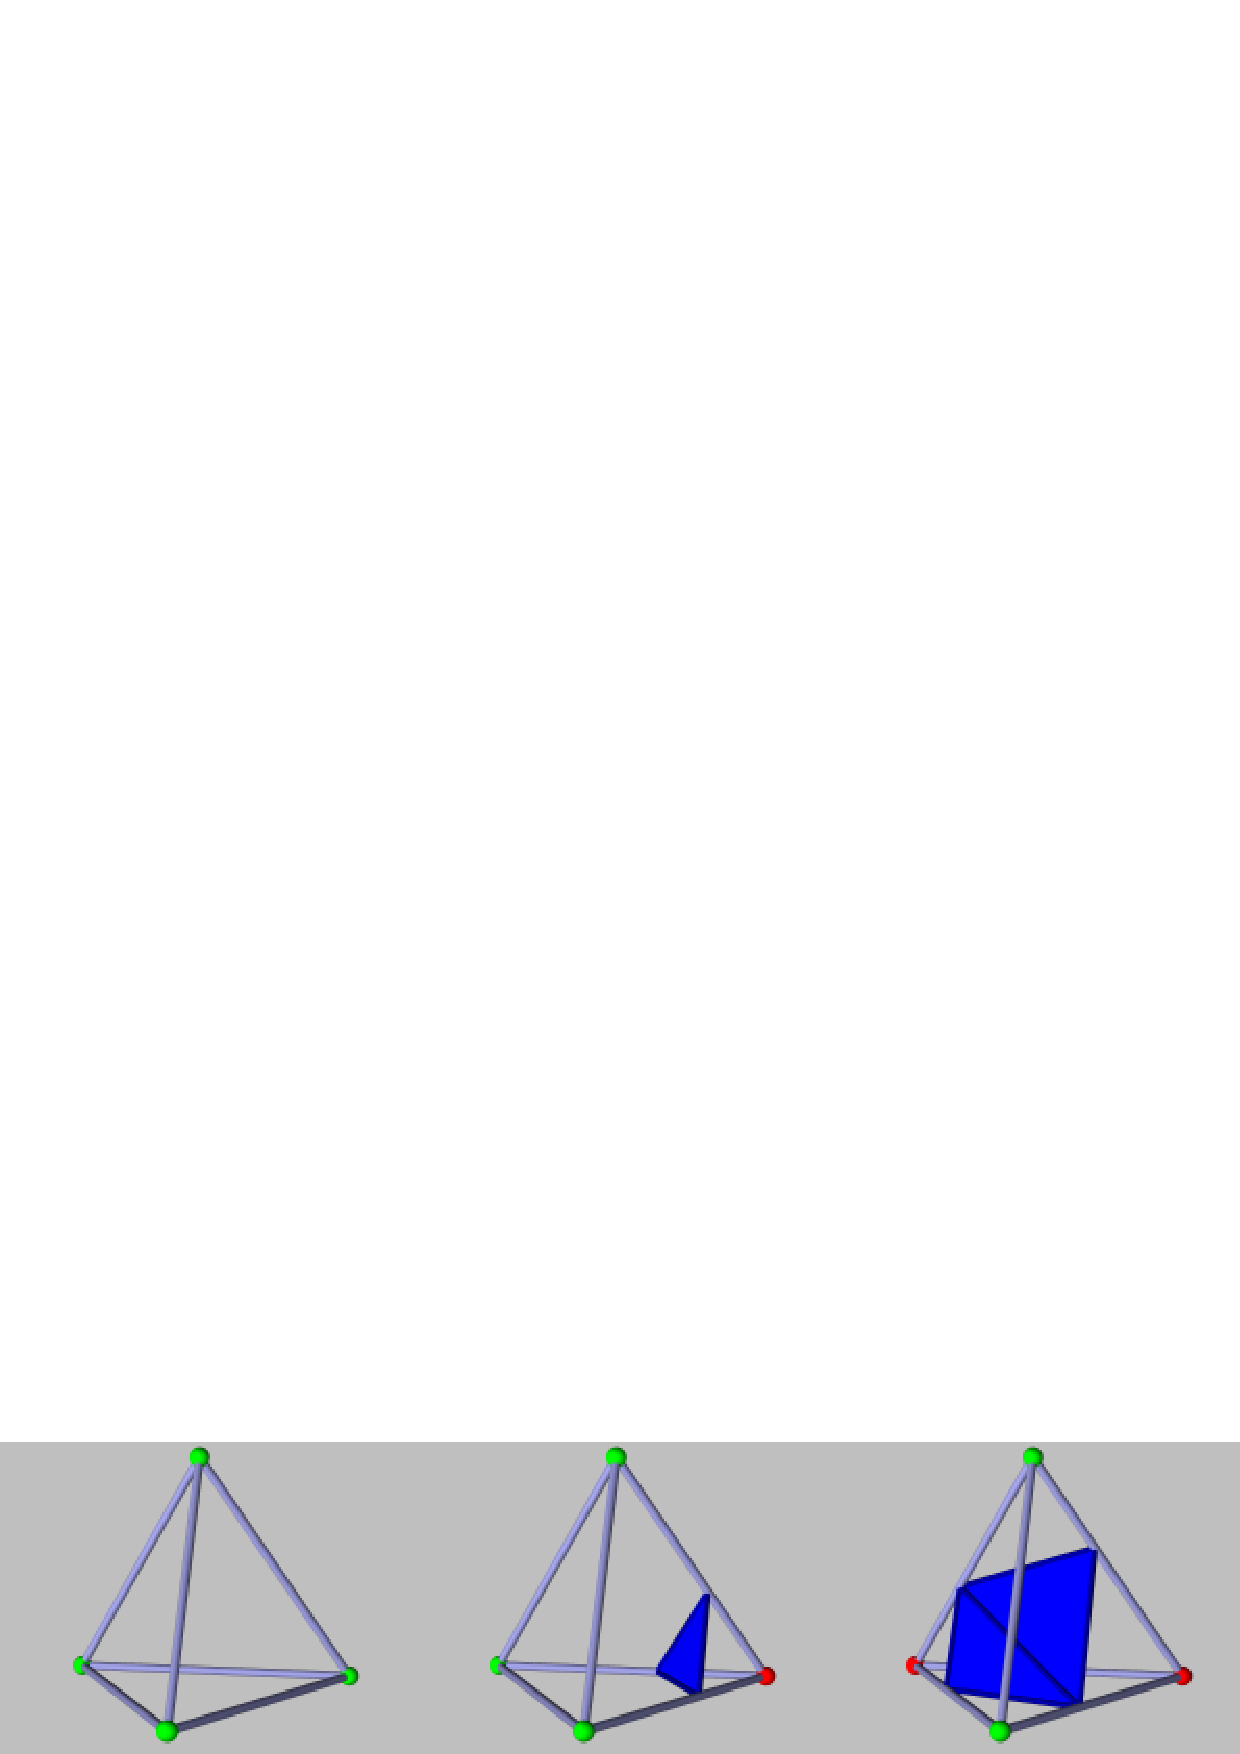
\includegraphics[width=.8\textwidth]{Skin_surface_3/marching}
\end{center}
\end{ccTexOnly}
\begin{ccHtmlOnly}
<CENTER>
<img border=0 src="./marching.png"
alt="Cases of the marching tetrahedra algorithm.">
</CENTER>
\end{ccHtmlOnly}

\caption{\label{SkinSurface3-fig-marching} Cases of the marching
  tetrahedra algorithm.}
\end{figure}

The function takes four arguments: the input triangulation, the
surface mesh, a policy class and an observer class.  The algorithm is
performed on the triangulation and the resulting mesh is stored in the
polyhedron. The \ccc{CGAL::Polyhedron_incremental_builder_3} is used
for constructing the polyhedron. There are two overloaded functions:

\ccGlobalFunction{template <class Triangulation_3,
                            class HDS,
                            class MarchingTetrahedraPolicy>
  void marching_tetrahedra_3(Triangulation_3 const t,
                             Polyhedron &p,
                             MarchingTetrahedraPolicy policy) ;}
\ccGlobalFunction{template <class Triangulation_3,
                            class HDS,
                            class MarchingTetrahedraPolicy,
                            class MarchingTetrahedraObserver>
  void marching_tetrahedra_3(Triangulation_3 const t,
                             Polyhedron &p,
                             MarchingTetrahedraPolicy policy,
                             MarchingTetrahedraPolicy observer) ;}

The policy class defines a predicate and a constructor. The predicate
is able to test whether a vertex of the triangulation lies inside or
outside the surface and the constructor is able to return the
intersection point of the surface with an edge of the triangulation
whose vertices lie on opposite sides of the surface. For skin surfaces
the intersection point is unique.

The observer class implements two functions that are called after the
construction of a vertex and a facet of the polyhedron. After
insertion of a vertex in the polyhedron a function is called with the
vertex of the polyhedron and the corresponding edge of the
triangulation. Similarly, after insertion of a facet in the polyhedron
a function is called with the facet of the polyhedron and the
corresponding cell of the triangulation. 

